\documentclass[tikz]{standalone}

\usetikzlibrary{shapes}
\usetikzlibrary{angles}
\usetikzlibrary{calc} 
    
\begin{document}

    
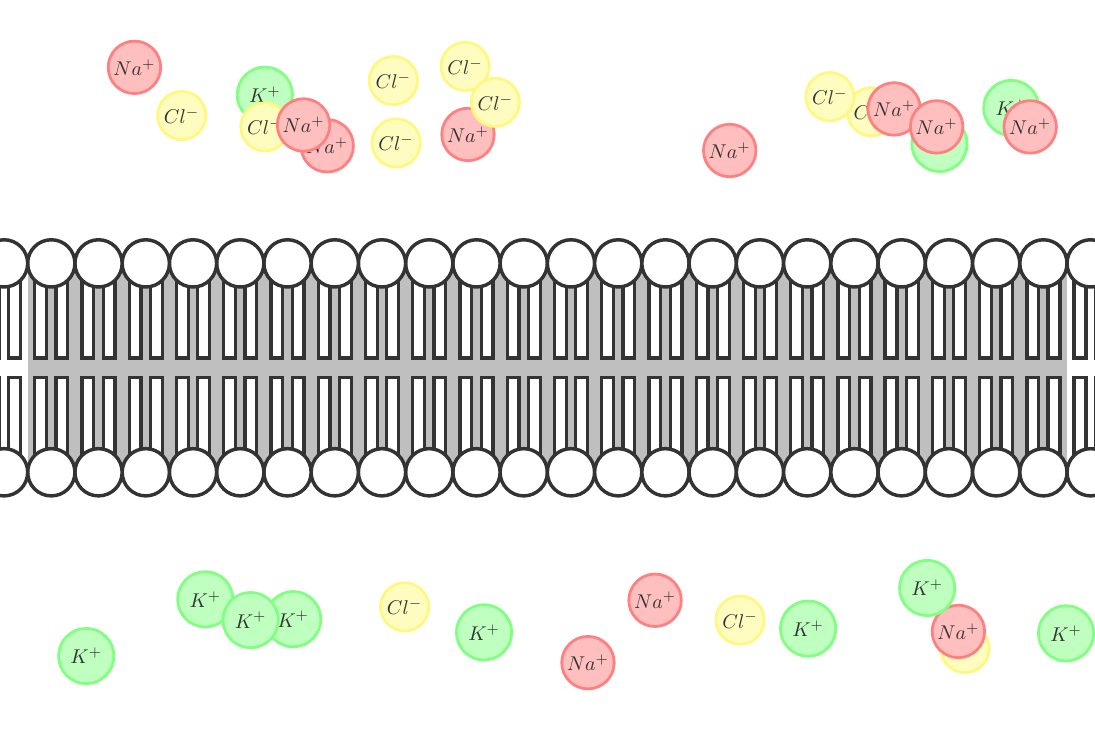
\begin{tikzpicture}[
    %x=1cm, y=1cm, 
    %z={(0cm,1cm)},
    scale = 1.2,
    transform shape,
    thick, 
    black!80,
    ]

    % Determines the boundries
    \path[use as bounding box] (-5.5,-3.6) rectangle (5.5,3.6);
    \fill[black!25] (-5.5,-1.2) rectangle (5.5,1.2);
    
    
    \def\linWid{1 pt}
    
    \def\r{0.5}             % radius of heads
    \def\s{0.5}             % scale
    \def\l{2}               % length
    \def\w{0.75}            % width
    \def\wl{1}              % width of the lipids
    \def\wc{1.30}           % width of the capacitor
    \def\j{2cm}             % not too sure
    \def\chanGap{3cm}
    \def\exShift{3}
    \def\steps{4}

    % Ratio for each ion
    \def\Nar{3/10}
    \def\Kr{7/10}
    \def\Lr{11.5/10}
    \def\Nas{Na}
    %\def\Kr{3/12}
    %\def\Nar{7/12}
    %\def\Nar{1/(2*\r*\s)}
    \def\Clr{11/12}
    
    % Random number generation seed
    \def\seed{22061999}
    
    % Random Num shit
    \def\randomX#1{\pgfmathrandominteger{#1}{-600}{600}}
    \def\randomY#1{\pgfmathrandominteger{#1}{225}{330}}

    
    % Definining the coordinates of the box corners
    \def\boxRise{2.2}
    \def\boxRun{3.75}
    
    \coordinate (O)  at (0,0);
    \coordinate (TR) at ( \boxRun, \boxRise);
    \coordinate (TL) at (-\boxRun, \boxRise);
    \coordinate (BL) at (-\boxRun,-\boxRise);
    \coordinate (BR) at ( \boxRun,-\boxRise);

    % Define centers of the walls of the circuit
    \coordinate (CC) at ($(TL)!1/2!(BL)$);
    \coordinate (LC) at ($(TR)!1/2!(BR)$);
    
    % Define centers of the floor and ceiling of the circuit
    \coordinate (EM) at ($(TL)!1/2!(TR)$);
    \coordinate (IM) at ($(BL)!1/2!(BR)$);

    \fill[red] ;

        
    \def\phosLipid#1{
        \draw [fill = white, line width = 1.20pt, transform shape] (#1)+(-0.35*\wl,0) rectangle +(-0.1*\wl,-\l);
        \draw [fill = white, line width = 1.20pt, transform shape] (#1)+(+0.35*\wl,0) rectangle +(+0.1*\wl,-\l);
        \draw [fill = white, line width = 1.25pt, transform shape] (#1) circle (\r);
    }

    \def\lipidBlock#1#2{
    \begin{scope}[xshift = #2]
        \begin{scope}[yshift = \exShift pt +\j*\s, scale = \s ]
            \foreach \i in {0,...,#1}{
                \phosLipid{ \i , 0 }
            }
        \end{scope}
        \begin{scope}[yshift = -\exShift pt -\j*\s, scale = \s, rotate = 180]
            \foreach \i in {0,...,-#1}{
                \phosLipid{ \i , 0  }
            }
        \end{scope}
    \end{scope}
    }

    % Maps out certain coordinates in relation to the centers of the channels
    \path ($(CC)!\Nar!(LC)$) node {}; \pgfgetlastxy{\Nax}{\Nay}
    \path ($(CC)!\Kr!(LC)$)  node {}; \pgfgetlastxy{\Kx}{\Ky}
    %\path (Na+) -- +(0:\w * 2 cm + 2 * 2 * \r*\s cm) node (Cl-) {};\pgfgetlastxy{\Clx}{\Cly}

    % The  lipids
    \foreach \Number/\Initial/\SIGN in {-11/ -1 /+,
                                         11/  1 /- }{
        \lipidBlock{\Number}{\Initial * \s cm \SIGN  \r * \s cm }
    }
    
    \begin{scope}
    % random scattering of ions in background
    \pgfmathsetseed{\seed}
    \foreach \CYC/\SIGN in {3/-1,8/+1}{
        \foreach \i in {1,...,\CYC}{
            \foreach \NN/\CC/\WW/\SS in 
                {K^+/green/227/-, 
                 Na^+/red/166/+, 
                 Cl^-/yellow/79/+}{
                    \pgfmathrandominteger{\rX}{-550}{550}
                    \pgfmathrandominteger{\rY}{228}{325}
                    
                    \draw (\rX/100,\SIGN * \SS\rY/100)  
                    node[circle, fill = \CC!25!white, draw = \CC!50, line width = 1pt, inner sep = 2*\WW/227, scale = 0.6] {$\phantom{Na^+}$}
                    node[scale = 0.6] {$ {\NN} $}; 
                }
        }}
    \end{scope}
\end{tikzpicture}


\end{document}